\documentclass[10pt,a4paper,onecolumn]{article}
\usepackage[left=0.75in, right=0.75in, top=1.00in, bottom=1.00in]{geometry}
\usepackage{url}
\usepackage{xcolor,colortbl}
\usepackage{hyperref}
\hypersetup{colorlinks=true,
linkcolor=red}
\usepackage{graphicx}
\definecolor{Gray}{gray}{0.85}

%opening
\title{Political Ideology Bias Detection with BERT}
\author{Ahsen Qamar and Alex Dauenhauer}

\begin{document}

\maketitle

\begin{abstract}
Abstract: TBD
\end{abstract}

\section{Introduction}
\label{intro}
\paragraph{}
Political ideology bias in news sources is a topic of growing concern, not just in the U.S., but across the entire world. As our country grows ever more partisan and misinformation campaigns fuel distrust in mainstream news sources, people have a tendency to turn to alternative news sources which typically reflect the existing ideology bias of the author. This creates echo chambers and reinforces existing partisan ideologies driving the partisan divide ever wider. The ability to automatically label biased text could inform readers that may have otherwise assumed the content was neutral, and encourage them to pursue alternative sources with less bias, or at the very least maintain a degree of skepticism about the content they are consuming. A system like this could also help media sources reduce the amount of bias they include their reporting, some of which may be unconscious and therefore undetected by writers or editors. Using this tool as a proofreader of sorts could eventually, hopefully reduce the amount of bias in media and reduce the growing partisan divide.

In this paper, we build off of previous work done by Iyyer et al. \cite{iyyerRNN}. Their success in using an RNN model to predict ideological bias at the sentence level, inspired us to expand on their experiments and attempt to improve on their performance using modern state-of-the-art tools such as BERT \cite{bert}. We use BERT for sequence classification to predict ideological bias at the sentence level on the Ideological Books Corpus as well as the Convote dataset, both of which are described in greater detail in section \ref{sec:data}. Additionally, we build a new dataset using news articles from 15 different publishers, with bias labels sourced from mediabiasfactcheck.com (MBFC) \cite{mbfc}. We predict bias at the sentence level, then use the aggregate sentence level predictions to predict bias at a document level and compare to the publisher label assigned by the MBFC team.

\section{Model \& Architecture}
\paragraph{}
BERT (Bidirectional Encoder Representations from Transformers) was released late last year by Google. The main draw towards the use of BERT for this project was leveraging the bi-directional training transformer to help detect political bias in text. For more information regarding BERT please refer to this \href{https://arxiv.org/abs/1810.04805}{research paper} from Google.

A cloud instance hosting an Nvidia P100 GPU was our environment for hosting our data as well as deploying our model for testing. This infrastructure limited us to use the BERT \textit{base} models. No significant difference was found between \textit{cased} and \textit{uncased} so we decided to move forward with \textit{BERT-Base, Cased}. The decision was made to move forward with a \textbf{pytorch} backend due to more thorough availability of code examples and better documentation. The primary reference for our code was from a \textit{Medium} article \cite{usingbert}.

Here is a high level diagram of our overall architecture:
\begin{figure}
	\begin{center}
		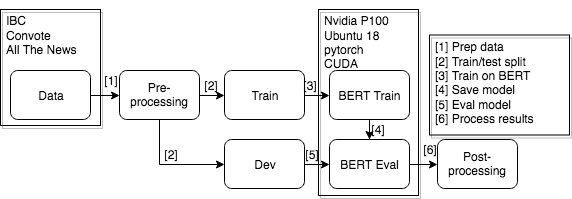
\includegraphics[width=0.8\linewidth]{architecture.png}
		\caption{Architecture}
		\label{fig:architecture}
	\end{center}
\end{figure}

\newpage

\section{Data}
\label{sec:data}
\paragraph{}
Political bias at the sentence level is a very subjective topic and therefore, there are not many large corpora widely available for use. A large part of this project was devoted to acquiring and preparing a few existing corpora, as well as repurposing a few processing methods on new corpora to develop our own biased sentence corpus. We performed experiments on three separate datasets: the Ideological Books Corpus (IBC) \cite{iyyerRNN}, Annotated congressional floor debates \cite{convote}, and the all-the-news dataset from Kaggle user Andrew Thompson \cite{news}. In this section we will describe the content of each dataset and processing steps performed on each dataset for use in our model.

\subsection{IBC}
\paragraph{}
The Ideological Books Corpus was provided to us in a fully processed format, courtesy of Iyyer et al.\cite{iyyerRNN} The original IBC dataset, developed by Gross et al.\cite{gross2013ibc} is a collection of books and articles written between 2008 and 2012 by well-known authors with strong political leanings. What Iyyer et al. did was to filter this corpus using a similar strategy to the strategy outlined in section \ref{sec:filtering}\footnote{Iyyer's team used bigrams and unigrams as their bias detectors, whereas we use trigrams and bigrams as ours}. They then crowd-sourced manual ideological bias annotations of the resulting sentences and particular subphrases. We use the data in this processed form as is, with no further processing.

\subsection{Convote}
\paragraph{}
The Convote dataset is a corpus of congressional speeches with each speech treated as a document with automatically derived labels of the speaker's political party (D, for Democrat; R, for Republican; I for Independent) as well as other related extracted information that was not pertinent to our experiments. Since our work attempts to predict ideological bias rather than political party, we relabel each document by mapping Democrat to "liberal", Republican to "conservative" and Independent to "neutral" (while we realize that a politician of Independent party certainly does not imply that politician's dialogue will be neutral, we use this label to select sentences that contain no bias detectors from either ideology which is explained further in section \ref{sec:filtering}). While it is true that the mapping of political party directly to political bias is not always a 1:1 relationship, there is a strong correlation between political party and political ideology. Further, we expect that our method for filtering the dataset for biased sentences will wash out noise that would be seen from speeches made by moderate centrists on either side of the aisle.

\subsubsection{Filtering Convote for Bias at the Sentence Level}
\label{sec:filtering}
\paragraph{}
It would be extremely unreasonable to assume that every sentence spoken by a member of congress during a congressional debate would contain ideological bias. In fact, a large portion of the sentences in the Convote dataset contain no bias at all.\footnote{Many sentences are simply opinion statements on whether or not the speaker agrees with the bill, or parliamentary jargon such as addressing the Speaker of the House, or urging their colleagues to vote a certain way, etc.} Therefore, it is necessary to filter this dataset for sentences that explicitly contain bias. 

To select the explicitly biased sentences from the dataset, we used a method inspired by Yano, et al. \cite{YanoBigrams} and shown to be successful as a bias identifier by Iyyer, et al. We started by identifying the most frequently used trigrams and bigrams for each label (liberal and conservative). We then filtered out any trigrams or bigrams which contained stopwords, and English names\footnote{Removing stopwords serves the purpose of eliminating trigrams and bigrams that don't contain substance for bias. Removing English names was a strategy that proved effective in filtering the all-the-news dataset, and was applied here as well, but essentially serves the purpose of removing n-grams that are sourced from replies to other speakers that address the other speaker by name}. We further filtered the bigrams list by requiring that at least one word in each bigram contain an "opinion" defined as a word found in the \texttt{opinion\_lexicon} corpus from NLTK\footnote{This method intends to select only those phrases that contain an ideological opinion which would typically be seen as a strong indicator of bias, when spoken by someone with known political affiliation. We decided to not make this a requirement for the trigrams as we felt these phrases would be unique enough to each ideology without this additional criteria that we did not want to lose information by filtering too heavily.}. We then took the set difference of the resulting top 1000 most frequent liberal and conservative n-grams (i.e. out of the top 1000 liberal bigrams, we only kept those that did not appear in the top 1000 conservative bigrams and vice versa, same for trigrams). We kept the top 100 filtered bigrams and top 100 filtered trigrams for each label as our bias indicators. We then filtered sentences such that, if a democratic speaker spoke a sentence that contained one of these top 200 "liberal" n-grams, we labeled that sentence as "liberal" and used the same logic applied to republican speakers to identify "conservative" sentences. For this dataset, we identified a neutral sentence as one which was spoken by an independent politician and contained no n-grams from either the liberal or conservative bias indicators. The top 10 n-grams from each label are shown in Table \ref{tab:ngrams-convote}. The resulting dataset included 1326 conservative sentences, 1383 liberal sentences and 213 neutral sentences. Example sentences from each ideology label are shown in Table \ref{tab:convote-sentences}.

\begin{table}[h!]
	\begin{center}
		\caption{Top 10 n-grams per ideology label - Convote}
		\label{tab:ngrams-convote}
		\begin{tabular}{p{0.2\linewidth}|p{0.2\linewidth}|p{0.2\linewidth}|p{0.2\linewidth}}
			\hline\hline
			\multicolumn{2}{c|}{\textbf{Liberal}} & \multicolumn{2}{c|}{\textbf{Conservative}} \\
			\hline
			Trigrams & Bigrams & Trigrams & Bigrams \\
			\hline
			social security trust & tax breaks & national electrical contractors & community protection \\
			security trust fund & security trust & electrical contractors association & free market \\
			cbc alternative budget & bad policy & legislative days within & organized crime \\
			black caucus budget & would lose & inner cell mass & bankruptcy relief \\
			estate tax relief & reduce crime & head start program & good news \\
			privatize social security & budget reconciliation & community protection act & relief extension \\
			u.s. trade deficit & ethical standard & million new jobs & delayed notification \\
			republican budget resolution & fiscally irresponsible & death tax repeal & soft money \\
			national wildlife refuge & working poor & 9/11 commission report & illegal aliens \\
			guardian ad litem & subpoena power & stem cells without & invasive species \\
			\hline\hline
		\end{tabular}
	\end{center}
\end{table}

\begin{table}[h!]
	\begin{center}
		\caption{Sample sentences from each ideology label - Convote}
		\label{tab:convote-sentences}
		\begin{tabular}{p{0.3\linewidth}|p{0.3\linewidth}|p{0.3\linewidth}}
			\hline\hline
			\textbf{Liberal} & \textbf{Conservative} & \textbf{Neutral}\\
			\hline
			mr. speaker, during a time of war, in the aftermath of a catastrophic hurricane, with 45 million americans lacking health insurance and skyrocketing home heating costs projected this winter, this majority is proposing to take from those with the least, give to those with the most -- and tell our children they will have to pay for it all later. & on both the business records and delayed notification sections of the patriot act (among others), the stance of the american civil liberties union and like-minded critics seems to have an ulterior motive. & let us look at what is going on in america today. \\
			it is clear that there would be plenty of money to deal with the social security trust fund if the president were not using the social security trust fund as a slush fund to give tax cuts to the wealthiest people in america. & that legislation helped to streamline the intelligence community and tightened some asylum rules that allowed potential terrorists to remain in our country. & mr. speaker, parliamentary inquiry. \\
			\hline\hline
		\end{tabular}
	\end{center}
\end{table}

\subsection{All-the-news Kaggle corpus}
\paragraph{}
To expand our training data further with a greater diversity of authors, we turned to a Kaggle corpus of 142,570 news articles from 15 different publishers as provided by Andrew Thompson \cite{news}. We assigned each publisher a bias label, sourced from mediabiasfactcheck.com (MBFC), then we simplified these labels down to the same labels we used in the previous datasets: liberal, conservative and neutral. The labels assigned to each publisher are shown in Table \ref{tab:pub-bias}. 

\begin{table}[h!]
	\begin{center}
		\caption{Publisher and bias labels from all-the-news corpus}
		\label{tab:pub-bias}
		\begin{tabular}{c|c|c}
			\hline\hline
			\textbf{Publisher} & \textbf{MBFC Bias Label} & \textbf{Simplified Bias Label} \\
			\hline
			New York Times & left-center & liberal \\
			\rowcolor{Gray}
			Breitbart & extreme-right & conservative \\
			\rowcolor{Gray}
			CNN & left & liberal \\
			Business Insider & left-center & liberal \\
			Atlantic & left-center & liberal \\
			\rowcolor{Gray}
			Fox News & right & conservative \\
			\rowcolor{Gray}
			Talking Points Memo & left & liberal \\
			Buzzfeed News & left-center & liberal \\
			National Review & right & conservative \\
			New York Post & right-center & conservative \\
			Guardian & left-center & liberal \\
			NPR & left-center & liberal \\
			Reuters & neutral & neutral \\
			\rowcolor{Gray}
			Vox & left & liberal \\
			Washington Post & left-center & liberal \\
			\hline\hline
		\end{tabular}
	\end{center}
\end{table}

\subsubsection{Filtering All-the-news for Bias at the Sentence Level}
\label{sec:filtering2}
\paragraph{}
Because the language used in a congressional debates is quite different than the language typically used in everyday journalism, the n-grams that we found in the Convote dataset don't crossover very well to the all-the-news dataset. Therefore we determine a new set of n-grams for the news article dataset. We applied a similar filtering method to the one explained in section \ref{sec:filtering} to filter sentences containing explicit bias. We first took a subset of publishers with the most extreme MBFC bias labels to determine biased n-grams from. This subset is indicated by the highlighted rows in Table \ref{tab:pub-bias}. From this subset, we selected n-grams that indicate bias similarly to the methods applied to the Convote set\footnote{We removed stopwords using a custom stopwords list, removed English names and required bigrams to include one "opinion" word. This is to remove boilerplate sentences, sentences that reference the author of a particular article and taglines such as "associated press", "bestselling author", "conservative columnist", etc.}. We kept the top 100 trigrams and bigrams, for a total set of 200 n-grams for each label, the top 10 of which are shown in Table \ref{tab:ngrams-atn}. Using these n-grams to select sentences that contained bias led to a dataset which contained 16,745 conservative sentences, 28,230 liberal sentences, 277,751 neutral sentences. To balance the dataset and avoid weighting strategies while training, we pared this down to a random selection of 16,000 sentences from each label, for a total of 48,000 sentences. 

\begin{table}[h!]
	\begin{center}
		\caption{Top 10 n-grams per ideology label - All-the-news}
		\label{tab:ngrams-atn}
		\begin{tabular}{p{0.2\linewidth}|p{0.2\linewidth}|p{0.2\linewidth}|p{0.2\linewidth}}
			\hline\hline
			\multicolumn{2}{c|}{\textbf{Liberal}} & \multicolumn{2}{c|}{\textbf{Conservative}} \\
			\hline
			Trigrams & Bigrams & Trigrams & Bigrams \\
			\hline
			senior administration official & opioid epidemic & jerusalem bureau chief & illegal aliens \\
			greenhouse gas emissions & health reform & border patrol agent & illegal alien \\
			north korean leader & lethal injection & social justice warriors & illegal immigrant \\
			federal civil rights & healthy people & black panther party & migrant crisis \\
			provocative narrative essays & racial bias & cartel chronicles project & patriot channel \\
			clean air act & budget reconciliation & refugee resettlement program & hard truths \\
			health care policy & chronic pain & prison sentence commuted & twin falls \\
			republican health care & lead poisoning & god less america & islamic terror \\
			gop health care & intelligence committees & real clear politics & snarky opinions \\
			civil rights laws & rights advocates & face certain death & dangerous faggot\footnotemark \\
			\hline\hline
		\end{tabular}
	\end{center}
\end{table}
\footnotetext{The extreme offensiveness of this bigram led us to investigate its origins further. The presence of this bigram is not actually due to conservative media using slurs like this commonly enough to rank in our top ten list. Instead it is actually a reference to "The Dangerous Faggot Tour" which is a campus speaking tour of Milo Yiannopoulos, a prominent contributor to Breitbart News. This is not to condone the use of this offensive slur, just to explain its origins and presence in this list a bit more clearly}

\begin{table}[h!]
	\begin{center}
		\caption{Sample sentences from each ideology label - All-the-news	}
		\label{tab:atn-sentences}
		\begin{tabular}{p{0.3\linewidth}|p{0.3\linewidth}|p{0.3\linewidth}}
			\hline\hline
			\textbf{Liberal} & \textbf{Conservative} & \textbf{Neutral}\\
			\hline
			Here’s what you need to know: American divisions are rapidly widening over President Trump’s order to close the U. S. to refugees and people from seven predominantly Muslim countries. & And the costs of illegal alien crime continued to mount and a lethal opioid epidemic raged. & Showcasing their attempts to unite with other groups for the election, Islamists campaigned with Awdeh Qawwas, a prominent priest, in the affluent Abdoun district of the capital Amman. \\
			In a video posted on her campaign’s Facebook page shortly after Mr. Sanders departed the White House grounds to visit the Capitol, Mr. Obama described Mrs. Clinton as the most qualified candidate to seek the White House, and implored Democrats to come together to elect her after a divisive party primary. & Obama’s claim of civic peace is also at odds with the televised evidence: dramatic race riots, cop killings, rapes, murders, illegal alien crimes, and chaos that rippled across the country during the second term of his presidency. & Rousseff’s survival hinges on winning over a dwindling number of undecided lawmakers who are also being courted by the man poised to take over if she is ousted, Vice President Michel Temer. \\
			\hline\hline
		\end{tabular}
	\end{center}
\end{table}

\section{Experiments/Results}
\paragraph{}
TBD after we run some experiments

\begin{table}[h!]
\centering
\caption{Accuracy Results Matrix}
\begin{tabular}{c||c|c|c|c||c} 
 \hline
 \textbf{Train/Test} & \textbf{IBC} & \textbf{Convote} & \textbf{AllTheNews} & \textbf{Documents} & \textbf{Evaluation Loss} \\ [0.5ex] 
 \hline\hline
 \textbf{IBC} & 60\% & 22.8\% & 40\% & N/A & 0.99 \\ 
 \textbf{Convote} & 20\% & 92.6\% & 63.5\% & 0\% & 0.23\\
 \textbf{AllTheNews} & 16.8\% & 60\% & 99.4\% & 65\% & 0.02 \\ [1ex]
 \hline
\end{tabular}
\label{table:results}
\end{table}

%\begin{table}[h!]
%\centering
%\begin{tabular}{||c c c c c||} 
% \hline
% \textbf{Train/Test} & \textbf{IBC} & \textbf{Convote} & \textbf{AllTheNews} & \textbf{Documents} \\ [0.5ex] 
% \hline\hline
% IBC & 60\% & 22.8\% & 40\% & N/A \\ 
% Convote & 20\% & 92.6\% & 63.5\% & 0\% \\
% AllTheNews & 16.8\% & 60\% & 99.4\% & 65\% \\ [1ex]
% \hline
%\end{tabular}
%\caption{Accuracy results matrix}
%\label{table:1}
%\end{table}
%
%\begin{table}[h!]
%\centering
%\begin{tabular}{||c c c c||} 
% \hline
% Metric & IBC & Convote & AllTheNews \\ [0.5ex] 
% \hline\hline
% Eval Loss & 0.99 & 0.23 & 0.02 \\ [1ex]
% \hline
%\end{tabular}
%\caption{Evaluation loss}
%\label{table:1}
%\end{table}

\section{Conclusion}
\paragraph{}
TBD

\section*{Future Research}
\paragraph{}
To expand on this project in the future, we would like to experiment with different bias detection methods in the source data. Use of n-grams with $ n > 3 $, alternative filtering methods such generating an opinion list customized to our dataset, or possibly investigating other techniques from the field of political science. 

To further develop this model and improve the usefulness of it at the document level, we would also like to incorporate BERT as an encoder in a Hierarchical Attention Network (HAN). In the most simplistic description, the HAN model encodes words into word vectors, then uses an attention mechanism to aggregate these into a sentence vector. Then the model repeats the process using the sentence vector with an attention mechanism to aggregate the sentences into a document vector for classification. We would like to incorporate BERT as our encoder in the HAN architecture which we believe would improve performance at the document level. We also will need to drastically improve the bias labels at the document level from the datasets we currently have available. This may involve a crowdsourcing task. Unfortunately we were not aware of the HAN model at the start of this project and when we found the architecture we did not have enough time to broaden our scope and incorporate it into this project.

\bibliographystyle{plain}
\bibliography{bibliography}

\end{document}
